\documentclass{article}
\usepackage[utf8]{inputenc}
\usepackage{enumitem}
\usepackage{geometry}
\usepackage{graphicx}
\usepackage{float}
\usepackage{listings}
\usepackage{hyperref}

\geometry{a4paper, margin=1in}

\lstset{
    basicstyle=\ttfamily\small,
    breaklines=true,
    frame=single,
    captionpos=b,
    xleftmargin=0.05\textwidth,
    xrightmargin=0.05\textwidth
}

\title{Research Assistant System}
\author{Team G.O.A.T\\
Abdelaziz Ibrahim, Besher Alkurdi, Bishwash Khanal}
\date{}

\begin{document}

\maketitle

\section{Agents' Roles and Behaviours}
\subsection{First scenario: Building Knowledge Base}

\subsubsection{Query Construction Agent}

\textbf{Role:} QueryFormulator | \textbf{Behaviour:} BDI Agent

\begin{itemize}
  \item Transforms natural language questions into optimized arXiv search syntax
  \item Creates multiple search strategies to increase coverage
  \item Handles both initial queries and refinement requests
  \item Sends queries to the Search Agent
  \item Receives refined queries and suggestions from the Relevant Agent
  \item \textbf{Goals:} \begin{itemize} 
    \item analyze\_query(Question)
    \item generate\_search\_params(Question)
    \item submit\_search\_request(Question, Queries)
    \item create\_refined\_search\_params(Question)
    \item submit\_refined\_search\_request(Question, Queries)
  \end{itemize}
\end{itemize}

\subsubsection{Search Agent}

\textbf{Role:} SearchCoordinator | \textbf{Behaviour:} Cyclic

\begin{itemize}
  \item Executes each query against the arXiv API
  \item Parses the results from arXiv API into a structured JSON format
  \item Forwards collected results to the Revelant Agent
\end{itemize}

\subsubsection{Relevant Agent}

\textbf{Role:} ResultValidator | \textbf{Behaviour:} BDI Agent

\begin{itemize}
  \item Evaluates the relevance of each paper against the research question
  \item Checks papers' relevance against a relevance threshold
  \item If the query is to be refined and only a few papers are relevant, send query refinement suggestions to the Query Construction Agent
  \item If sufficient papers are returned, send the papers to the Knowledge Agent
  \item \textbf{Goals:} \begin{itemize} 
    \item evaluate\_paper\_relevance(Question, Results)
    \item decide\_next\_action(Question)
    \item request\_query\_refinement(Question)
    \item forward\_relevant\_papers(Question)
  \end{itemize}
\end{itemize}

\subsubsection{Knowledge Aggregator Agent}

\textbf{Role:} ContentCollector | \textbf{Behaviour:} BDI Agent

\begin{itemize}
  \item Receives papers info from the Relevant Agent
  \item Deduplicates the received papers
  \item Saves the results (Papers info) as a JSON file to create a knowledge base
  \item \textbf{Goals:} \begin{itemize} 
    \item create\_knowledge\_base(Question, Papers)
    \item process\_paper\_content(Papers)
    \item save\_research\_data
    \item notify\_analysis\_agent
  \end{itemize}
\end{itemize}

\subsection{Second scenario: Analyzing Papers}

\subsubsection{Analysis Agent}

\textbf{Role:} AnalyzePapers | \textbf{Behaviour:} OneShot

\begin{itemize}
  \item Retrieves the specified papers' content using JINA API
  \item Extracts the methodology, findings and future work from each paper
  \item Saves the extracted information in a structured format (JSON)
  \item Sends the structured data to the Synthesis Agent
\end{itemize}

\subsubsection{Synthesis Agent}

\textbf{Role:} SynthesizeReport | \textbf{Behaviour:} OneShot

\begin{itemize}
  \item Uses the extracted information from the Analysis Agent
  \item Extracts common themes, research gaps, and suggested future work from the papers
  \item Generates a comprehensive report summarizing the findings
  \item Saves the extracted information in a structured format (JSON)
\end{itemize}

\section*{Agent's Communication (Sequence Diagram)}

\begin{figure}[H]
    \centering
    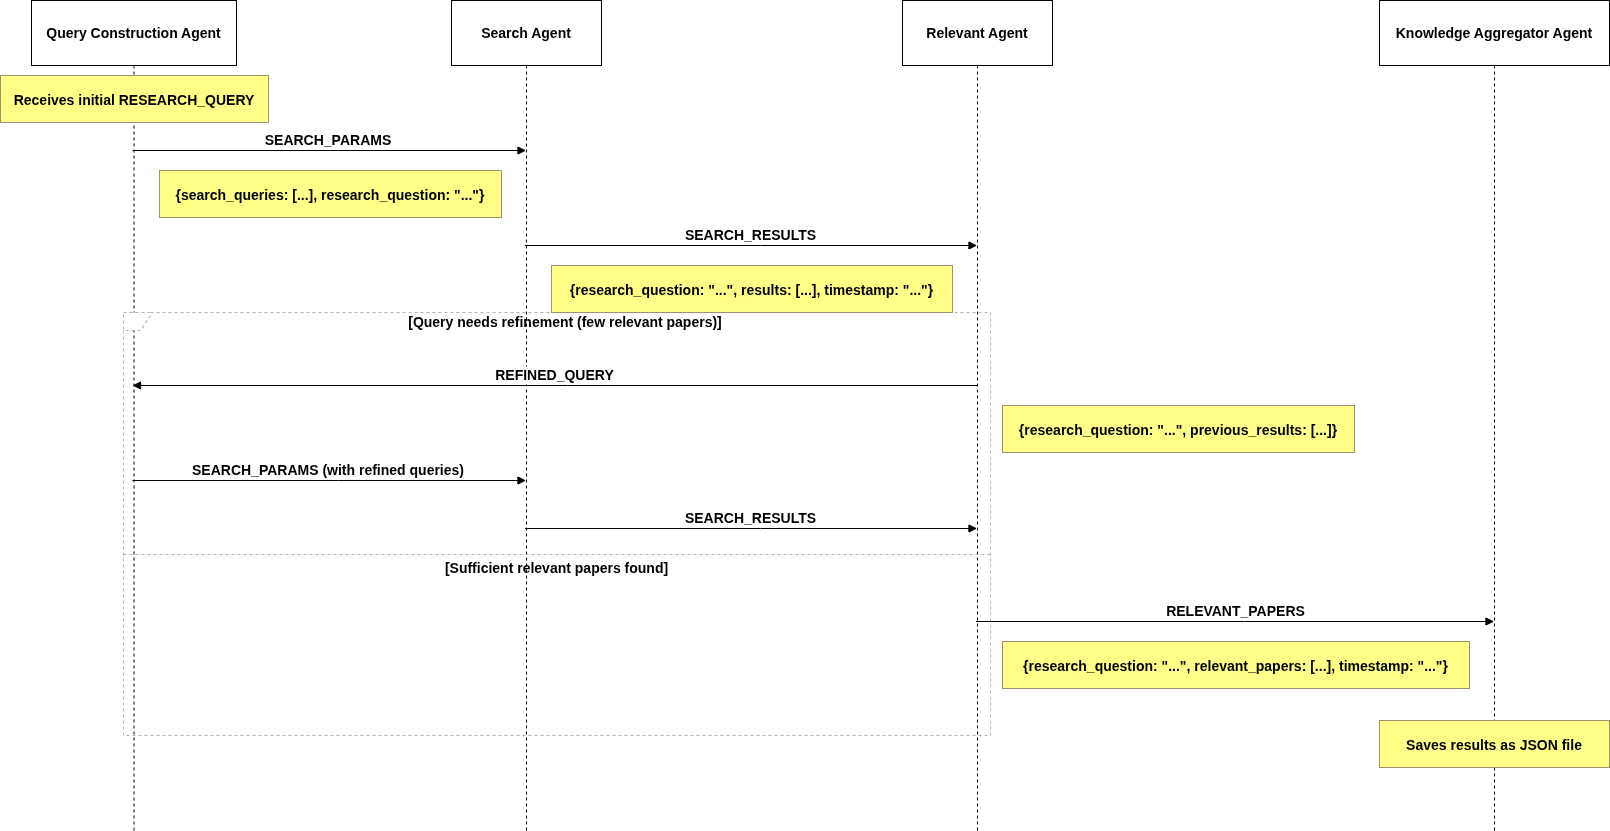
\includegraphics[width=\textwidth]{images/agent_communication.png}
    \caption{First Scenario Sequence Diagram}
    \label{fig:First-Scenario}
\end{figure}

\begin{figure}[H]
    \centering
    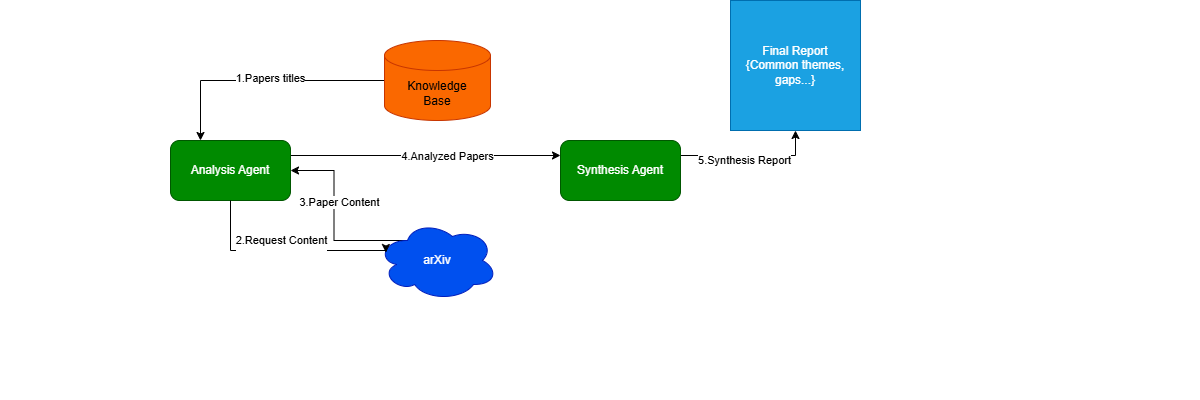
\includegraphics[width=\textwidth]{images/agents.drawio.png}
    \caption{Second Scenario Block Diagram}
    \label{fig:Second-Scenario}
\end{figure}



\section*{Screenshots}

\begin{figure}[H]
    \centering
    \includegraphics[width=\textwidth]{images/Screenshot_1.png}
    \caption{Agent Console Output 1}
    \label{fig:screenshot1}
\end{figure}

\begin{figure}[H]
    \centering
    \includegraphics[width=\textwidth]{images/Screenshot_2.png}
    \caption{Agent Console Output 2}
    \label{fig:screenshot2}
\end{figure}

\begin{figure}[H]
    \centering
    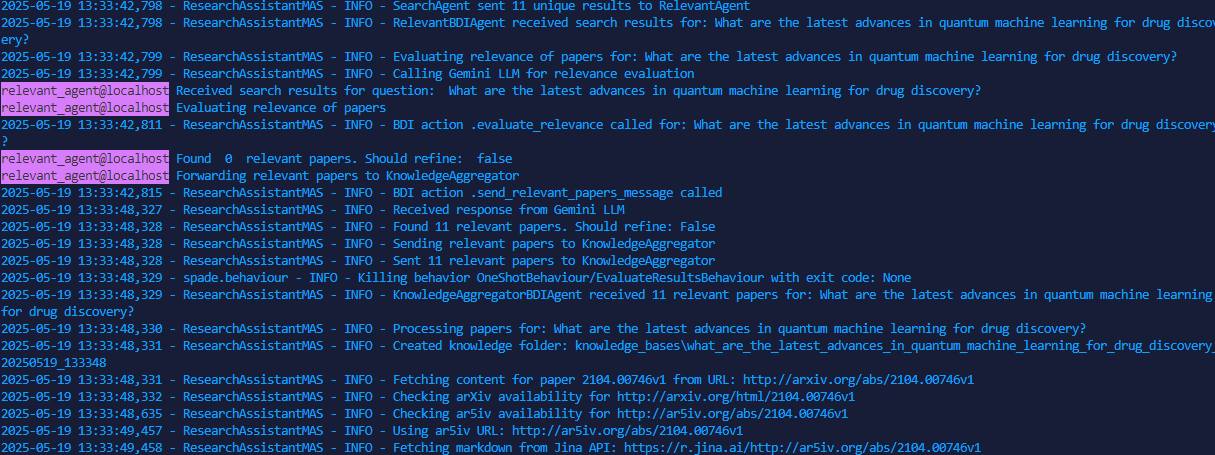
\includegraphics[width=\textwidth]{images/Screenshot_3.png}
    \caption{Agent Console Output 1}
    \label{fig:screenshot3}
\end{figure}

\begin{figure}[H]
    \centering
    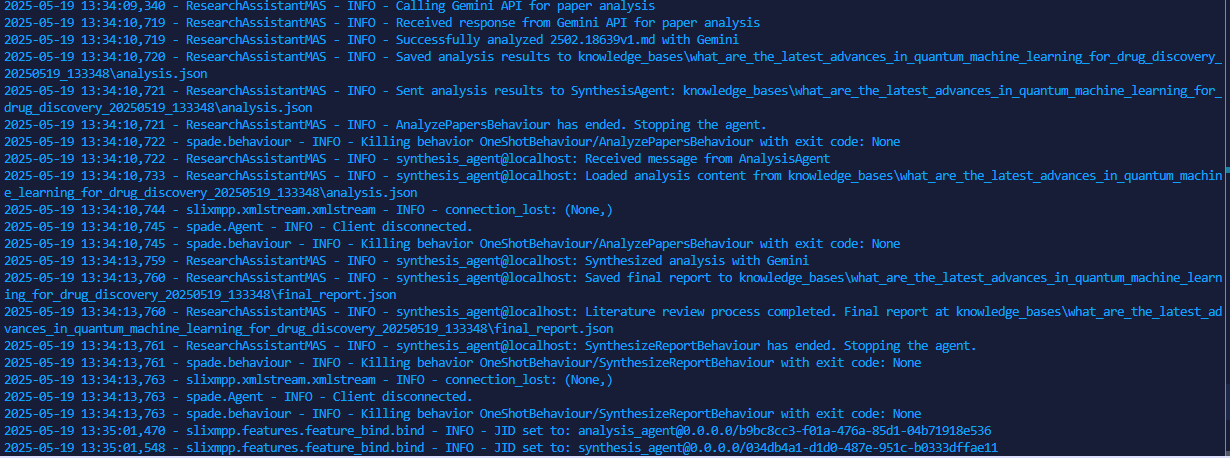
\includegraphics[width=\textwidth]{images/Screenshot_4.png}
    \caption{Agent Console Output 2}
    \label{fig:screenshot4}
\end{figure}

\section*{GitHub Repository}
The source code for this project is available on GitHub:
\begin{center}
  \url{https://github.com/bkhanal-11/agentic_technologies_project}
\end{center}

\end{document}